%! TeX root = master.tex
% !TEX program = lualatex

\lecture{2}{2026-09-16}{Bandit Model and Probability Review}{}

\section{Multi-Armed Bandits}

\subsection{A bit of history and motivation}

The name ``bandit'' comes from the slot machine: pulling an arm yields a reward (minus the investment), and $\mathbb{E}[\text{payoff}] < 0$ -- hence a ``bandit''. In the old days, a slot machine used a mechanical random number generator; different machines (``one-armed bandits'') can behave subtly differently. The fundamental question is: \emph{which arm to pull}? In particular, if we play for a long time but know nothing at the beginning, how do we use the information gathered along the way optimally?

The field was initiated by William R.\ Thompson [\textit{Biometrika}, 1933], motivated by clinical trials: sequential decision-making under uncertainty, aiming to minimize unnecessary harm to patients. Bandit models have many applications in online services, where there is a lot of data, a lot of decisions to make, and human intervention is generally not feasible.

\begin{remark}
The objective of this course is to extract \emph{principles}: clean ``vignettes'' of often messier real-world situations, chosen for their mathematical tractability. The algorithms studied are not necessarily directly applicable to all real-world situations, but the underlying principles are tools that guide the design of real-world solutions.
\end{remark}

\subsubsection*{Real-world examples}

\begin{itemize}
    \item \textbf{A/B-testing web interfaces}: automate design choices for web/online interfaces; reward = user traffic, activity, engagement time, etc.
    \item \textbf{Ad placement}: place ads at the right location and show the right ad at the appropriate time; reward = ad revenue.
    \item \textbf{News recommendations}: serve news stories of interest to every user; reward = clicks, engagement time, etc.
    \item \textbf{Dynamic pricing}: optimize price over time so as to sell the full inventory while maximizing revenue; reward = total revenue.
    \item \textbf{Monte Carlo Tree Search (MCTS)}: used in recent successes of ML approaches to game playing (Atari games, chess, Go, \dots). A tree captures positions already explored; the algorithm generates a path down the known tree, expands a leaf, plays randomly to the end, and propagates the reward back up. Conceptually, every node contains a bandit algorithm that learns rewards ``further down'' based on the choice of child node. Over time, higher-reward paths get chosen more often, while uncertainty is still handled explicitly.
\end{itemize}

\subsubsection*{Back to the clinical trial example: what might go wrong?}

With a purely randomized test, each patient randomly receives the drug or the placebo. At the end of the trial, effectiveness is assessed, e.g., via a hypothesis test: fix a $p$-value (e.g., $0.05$) and a criterion (e.g., probability of recovery twice as high as without treatment); this determines the necessary number of samples. The trial is carried out, then evaluated -- success or failure.

The issue: nothing is done \emph{during} the trial. What if, after only a short time, the data already show a strongly imbalanced outcome between the two arms?

This motivates a \emph{sequential} approach, where decisions can be updated as data comes in, rather than fixed in advance.

\newpage
\begin{parag}{Reminder: p-value}
    A hypothesis test is a probabilistic proof by contradiction. We fix a \textbf{null hypothesis} $H_0$ (the status quo, e.g.\ ``the new treatment is no better than the old one'') and an \textbf{alternative hypothesis} $H_1$ (what we want to show, e.g.\ ``the new treatment is better'').

    Given a test statistic $T$ (e.g.\ the number of cured patients) with observed value $t_{\text{obs}}$, the \textbf{p-value} is the probability, \textit{assuming $H_0$ is true}, of observing a result at least as extreme as the one we observed:
    \[p = \prob\left(T \geq t_{\text{obs}} \mid H_0\right)\]

    \textbf{Decision rule.} We fix a significance level $\alpha$ \textit{before} looking at the data (typically $\alpha = 0.05$):
    \begin{itemize}
        \item If $p \leq \alpha$: we \textbf{reject $H_0$}, and the result is statistically significant.
        \item If $p > \alpha$: we \textbf{fail to reject $H_0$}. This does \textit{not} mean that $H_0$ is true, only that the data does not provide enough evidence against it.
    \end{itemize}

    \textbf{Errors.}
    \begin{itemize}
        \item \textbf{Type I error} (false positive): rejecting $H_0$ while it is true. By construction, this happens with probability $\alpha$.
        \item \textbf{Type II error} (false negative): not rejecting $H_0$ while it is false. This happens with probability $\beta$, and $1 - \beta$ is called the \textbf{power} of the test.
    \end{itemize}
\end{parag}

\subsection{Stochastic bandits: definitions, assumptions, vocabulary}

The basic interaction loop is as follows: the \textbf{learner/agent} takes actions $A_i$, and the \textbf{environment} generates rewards $X_i$, over a \textbf{horizon} $n$:
\[
A_1, X_1, A_2, X_2, A_3, X_3, \dots, A_n, X_n.
\]
\begin{center}
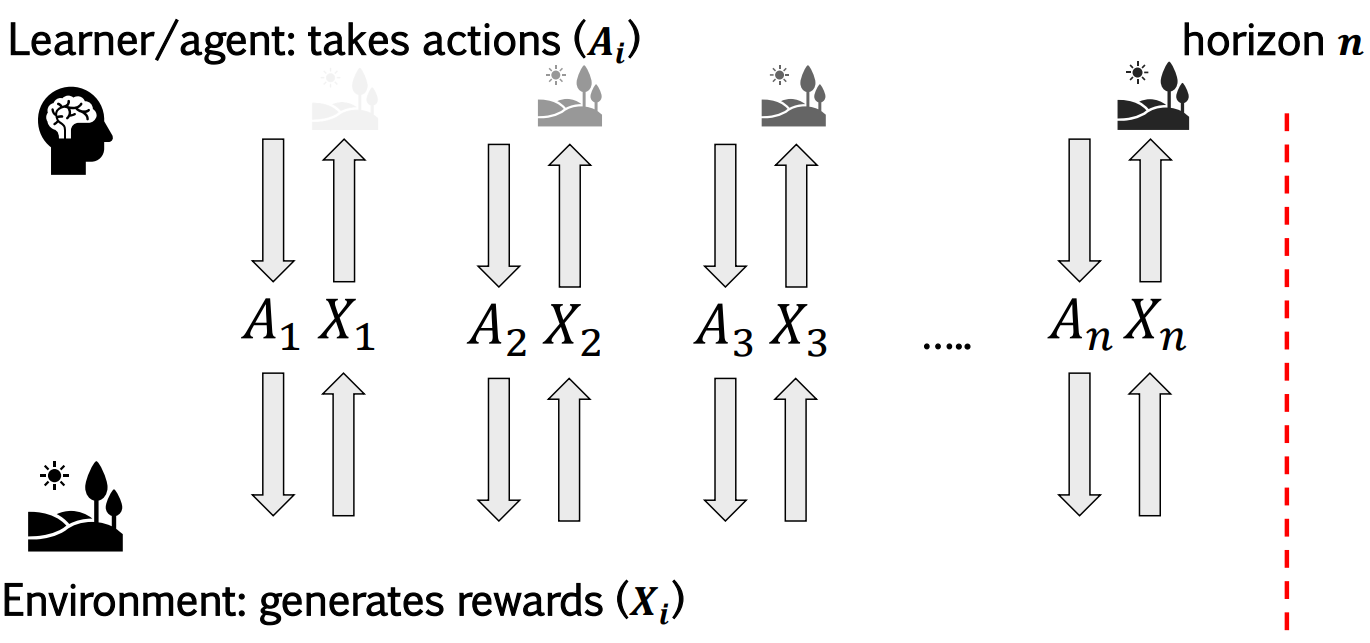
\includegraphics[width=0.6\linewidth]{images/img_20260920_120748.png}
\end{center}

\begin{definition}[History]
The history up to time $t$ is $H_t = (A_1, X_1, A_2, X_2, \dots, A_t, X_t)$. It contains all the information the learner has so far about the environment.
\end{definition}

\begin{definition}[Policy]
A policy $\pi$ is a map from history to action: $A_t = \pi(H_{t-1})$. More specifically, the action can be random: $\pi_t$ is a conditional distribution over $A_t$ given $A_1, X_1, A_2, X_2, \dots, A_{t-1}, X_{t-1}$ (but it cannot depend on the future).
\end{definition}

\begin{definition}[Environment]
The environment is a map from $A_1, X_1, A_2, X_2, \dots, A_t$ to $X_t$ (possibly random).
\end{definition}

\textbf{Goal.} Maximize the cumulative reward up to the horizon $n$: $S_n = \sum_{i=1}^n X_i$.

\begin{remark}[Key assumption]
The learner does \emph{not} know the environment at the beginning, although it might know some \emph{class} of possible environments.
\end{remark}

\begin{definition}[Regret]
The regret of the learner relative to a policy $\pi^*$ is the expected reward under $\pi^*$ minus the expected reward achieved by the learner -- the ``cost of ignorance''. Usually, $\pi^*$ is the optimal policy for the environment, i.e., a policy that knows the environment perfectly.
\end{definition}

\subsection{Unstructured vs.\ structured bandits}

\begin{definition}[Unstructured bandit]
Intuitively, an unstructured bandit is one where pulling one arm provides no information on the reward distribution of other arms. Formally, the environment class is
\[
\mathcal{E} = \left\{ \nu = (P_a : a \in \mathcal{A}) : P_a \in \mathcal{M}_a \text{ for all } a \in \mathcal{A} \right\},
\]
where $\mathcal{M}_a$ is a family (set) of possible distributions $P_a$ for action $a$. In other words, $\mathcal{E} = \bigtimes_{a \in \mathcal{A}} \mathcal{M}_a$ is a \emph{product space}: any combination of elements from the $\mathcal{M}_a$'s is possible. This ensures that knowing anything about $P_a$ provides no information about $P_{a'}$ for $a' \neq a$.
\end{definition}

\begin{framedremark}
    The objects in this definition live at different levels:
    \begin{itemize}
        \item $P_a$ is \textbf{one} distribution: the true (unknown) reward distribution of arm $a$, e.g.\ $\text{Ber}(0.7)$.
        \item $\mathcal{M}_a$ is a \textbf{set} of distributions: all candidates that $P_a$ could be, i.e.\ what we assume about arm $a$ before playing. For instance, $\mathcal{M}_a = \{\text{Ber}(p) : p \in [0,1]\}$ (binary rewards), $\mathcal{M}_a = \{\mathcal{N}(\mu, 1) : \mu \in \R\}$ (Gaussian with known variance), or all distributions supported on $[0,1]$ (bounded rewards).
        \item $\nu = (P_a : a \in \mathcal{A})$ is a \textbf{tuple} of distributions, one per arm: it is \textit{one} specific environment, e.g.\ $\nu = (\text{Ber}(0.7), \text{Ber}(0.4))$.
        \item $\mathcal{E}$ is a \textbf{set} of environments: all those consistent with our assumptions.
    \end{itemize}
    The learner does not know $\nu$ (this is what it must learn), it only knows that $\nu \in \mathcal{E}$. Learning amounts to progressively narrowing down the candidates in each $\mathcal{M}_a$ until $P_a$ is identified well enough. The guarantees of an algorithm hold only if the true $P_a$ indeed belongs to the assumed $\mathcal{M}_a$.
\end{framedremark}

\subsubsection*{Examples of unstructured bandit classes}

\begin{center}
\begin{tabular}{lll}
\hline
Name & Parametric & Definition \\
\hline
Bernoulli & Yes & $\mathcal{B}(\mu_i)$, $\mu_i \in [0,1]$ \\
Uniform & Yes & $\mathcal{U}(a_i, b_i)$, $a_i \leq b_i \in \mathbb{R}$ \\
Gaussian, known variance & Yes & $\mathcal{N}(\mu_i, \sigma^2)$ \\
Gaussian, unknown variance & Yes & $\mathcal{N}(\mu_i, \sigma_i^2)$ \\
Finite variance & No & $\mathbb{V}(P_i) \leq \sigma^2$ \\
Bounded support & No & $\mathrm{Supp}(P_i) \subseteq [a,b]$ \\
Subgaussian & No & $P_i$ is $\sigma$-subgaussian \\
\hline
\end{tabular}
\end{center}

\begin{definition}[Structured bandit]
Intuitively, a structured bandit has an environment class where the reward of one arm provides information on the reward distribution of other arms.
\end{definition}

\textbf{Examples.}
\begin{itemize}
    \item \emph{``Complementary Bernoulli'' bandit}: $\mathcal{A} = \{1, 2\}$, $\mathcal{E} = \{(\mathcal{B}(\theta), \mathcal{B}(1-\theta)) : \theta \in [0,1]\}$. One could learn everything by playing only one arm forever. Example: two mutually exclusive options to click on a webpage.
    \item \emph{Stochastic linear bandit}: $\mathcal{A} \subset \mathbb{R}^d$ (an uncountably infinite action space), $\theta \in \mathbb{R}^d$, $\mathcal{E} = \{\nu_\theta : \theta \in \mathbb{R}^d\}$ with $\nu_\theta = \{\mathcal{N}(\langle a, \theta \rangle, 1) : a \in \mathcal{A}\}$. Example: a recommender system, where $\theta$ captures unknown user preferences and $a$ captures the feature vector of an item; $\langle a, \theta \rangle = a^T \theta$ is the inner product measuring how much the user likes item $a$.
  \begin{center}
    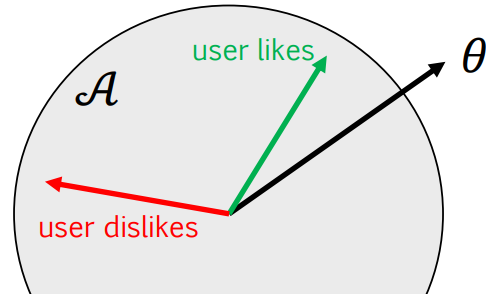
\includegraphics[width=0.3\linewidth]{images/img_20260920_131516.png}
  \end{center}

\end{itemize}

\subsubsection*{Thought experiment: the case of no noise}

In this idealized setting, we assume that pulling an arm reveals its \emph{exact} expected reward, rather than a noisy sample drawn around it: $r_t = \mu_a$ instead of $r_t = \mu_a + \varepsilon_t$. In other words, a single pull gives perfect information about the arm's true mean, with no randomness to average out. This is of course unrealistic (real feedback is always noisy), but it is a useful thought experiment to understand how much easier the bandit problem becomes once uncertainty is removed.

\begin{itemize}
    \item \textbf{Unstructured bandit}: try each of the $k$ arms once, observe a (deterministic) reward, then play the best arm forever -- no more regret is incurred afterwards; the cumulative regret is constant.
    \item \textbf{Structured bandit}: e.g., in the complementary Bernoulli case, there is one permanent winner and one permanent loser, so pulling once suffices to be perfect forever. In the stochastic linear case, getting exact inner products (i.e., projections) requires that the set of actions spans $\mathbb{R}^d$; then $d$ pulls suffice to estimate $\theta$ perfectly.
\end{itemize}

This noiseless setting is not very interesting, nor realistic in most practical settings. \textbf{The main topic in bandit theory is dealing with noise in the reward}, which gives rise to a non-zero expected regret ``forever''.

\subsection{Review of some probability notions}

\subsubsection*{CDF, CCDF, density}

For a continuous random variable $A$:
\[
F_A(a) = \mathbb{P}(A \leq a), \qquad F'_A(a) = \mathbb{P}(A > a) = 1 - F_A(a) \ \text{(CCDF)}, \qquad f_A(a) = \frac{dF_A(a)}{da} \geq 0.
\]

\subsubsection*{Independence}

Two random variables are independent iff $F_{A,B}(a,b) = F_A(a)F_B(b)$ for all $a,b$: information on one variable provides no information on the other.

A set of random variables is \textbf{pairwise independent} iff every pair is independent. A set of random variables is \textbf{mutually independent} iff $F_{A,B,C}(a,b,c) = F_A(a)F_B(b)F_C(c)$ (for three variables; analogously for more): any information on all the other variables provides no information on a target variable.

\begin{remark}
Mutual independence is \emph{strictly stronger} than pairwise independence!
\end{remark}

\begin{example}
Let $A, B \sim \mathcal{B}(1/2)$ i.i.d., and let $C = A \oplus B$ (XOR). Contrast the two joint laws below (left: $A,B,C$ constructed this way; right: $A,B,C \sim \mathcal{B}(1/2)$ i.i.d.\ and mutually independent):

\begin{center}
\begin{tabular}{cc}
$\begin{array}{c|c}
ABC & \mathbb{P} \\
\hline
000 & 1/4 \\
001 & 0 \\
010 & 0 \\
011 & 1/4 \\
100 & 0 \\
101 & 1/4 \\
110 & 1/4 \\
111 & 0
\end{array}$
&
$\begin{array}{c|c}
ABC & \mathbb{P} \\
\hline
000 & 1/8 \\
001 & 1/8 \\
010 & 1/8 \\
011 & 1/8 \\
100 & 1/8 \\
101 & 1/8 \\
110 & 1/8 \\
111 & 1/8
\end{array}$
\end{tabular}
\end{center}

In the XOR construction, every \emph{pair} $(A,B)$, $(A,C)$, $(B,C)$ is uniform on $\{0,1\}^2$ with all four combinations having probability $1/4$ -- i.e., every pair is independent. However, the three variables are \emph{not} mutually independent: knowing any two of them determines the third exactly.
\end{example}

\subsubsection*{Conditional independence}

\begin{definition}
$A$ and $B$ are conditionally independent given $C$ iff, in the discrete case,
\[
\mathbb{P}(A \leq a, B \leq b \mid C = c) = \mathbb{P}(A \leq a \mid C = c)\, \mathbb{P}(B \leq b \mid C = c) \quad \text{for all } a,b,c \ (\mathbb{P}(C=c) > 0),
\]
or, in the continuous case, $f_{AB \mid C}(a,b \mid c) = f_{A \mid C}(a \mid c)\, f_{B \mid C}(b \mid c)$ for all $a,b,c$ (with $f_C(c) > 0$).
\end{definition}

Intuitively: if $C$ is known, then $A$ provides no further information about $B$ (and vice versa). The notions of pairwise and mutual independence also extend naturally to conditional independence when there are more than two variables.

\subsubsection*{Expectation}

\[
\mathbb{E}[X] = \mu_X = \begin{cases} \sum_{x_i} x_i\, \mathbb{P}(X = x_i) & \text{discrete} \\ \int x f_X(x)\, dx & \text{continuous} \end{cases}
\]

Some important properties:
\begin{itemize}
    \item \textbf{Linearity}: $\mathbb{E}[A + B] = \mathbb{E}[A] + \mathbb{E}[B]$ for any $A, B$.
    \item \textbf{Product}: $\mathbb{E}[AB] = \mathbb{E}[A]\,\mathbb{E}[B]$ if $A \perp B$, but this is \emph{not} true in general.
    \item For $A \geq 0$: $\mathbb{E}[A] = \int_0^\infty F'_A(x)\, dx$ (integral of the CCDF).
    \item $\mathbb{E}[\mathbf{1}\{E\}] = \mathbb{P}(E)$, where $\mathbf{1}(E)$ is the indicator of event $E$.
\end{itemize}

\subsubsection*{Conditional expectation}

\begin{definition}
$\mathbb{E}[A \mid B = b] = \sum_a a\, \mathbb{P}(A = a \mid B = b) =: f(b)$, and $\mathbb{E}[A \mid B] = f(B)$. Note that this is a \emph{random variable} in $B$.
\end{definition}

\begin{example}
Let $B \sim \mathcal{U}(0,1)$ and $A \sim \mathcal{B}(B)$ (i.e., a Bernoulli whose parameter is itself the random variable $B$). Then $\mathbb{E}[A \mid B] = B$.
\end{example}

Further properties:
\begin{itemize}
    \item If $A \perp B$, then $\mathbb{E}[A \mid B] = \mathbb{E}[A]$.
    \item ``Pulling out what is known'': $\mathbb{E}[A\, g(B) \mid B] = g(B)\, \mathbb{E}[A \mid B]$, since conditional on $B = b$, $g(B) = g(b)$ is a constant and can be pulled in front of the sum/integral.
    \item \textbf{Tower property (law of total expectation)}: $\mathbb{E}[\mathbb{E}[A \mid B]] = \mathbb{E}[A]$.
\end{itemize}

\begin{example}[Using the tower property]
Let $C \sim \mathrm{Unif}(-1,1)$, and let $A = \mathcal{N}(C,1)$, $B = \mathcal{N}(C,1)$, with $A \perp B \mid C$ (i.e., $A - C - B$ forms a Markov chain). Note that $A$ and $B$ are \emph{dependent} (even though conditionally independent given $C$). Suppose we need to compute $\mathbb{E}[AB]$. Rather than computing the joint density $f_{AB}(a,b)$ and integrating $\iint ab\, f_{AB}(a,b)\, da\, db$, we can use the tower property:
\[
\mathbb{E}[AB] = \mathbb{E}\big[\mathbb{E}[AB \mid C]\big].
\]
By conditional independence, $\mathbb{E}[AB \mid C = c] = \mathbb{E}[A \mid C=c]\,\mathbb{E}[B \mid C=c] = c^2$. Hence
\[
\mathbb{E}\big[\mathbb{E}[AB \mid C]\big] = \mathbb{E}[C^2] = \int_{-1}^{1} \frac{1}{2} c^2\, dc = \frac{1}{3}.
\]
\end{example}

\subsection{Back to bandits: regret}

\begin{definition}[Expected and maximum reward]
For a stochastic bandit given by $\nu = (P_a : a \in \mathcal{A})$, the expected reward of arm $a$ is
\[
\mu_a(\nu) = \int_{-\infty}^{+\infty} x\, dP_a(x) = \mathbb{E}[X], \quad X \sim P_a,
\]
and the maximum expected reward is $\mu^*(\nu) = \max_{a \in \mathcal{A}} \mu_a(\nu)$.
\end{definition}

\begin{definition}[Regret]
The regret of policy $\pi$ on bandit instance $\nu$ is
\[
R_n(\pi, \nu) = n\mu^* - \mathbb{E}\left[\sum_{t=1}^n X_t\right].
\]
Note that the regret is \emph{not} a random quantity (the randomness has already been integrated out via the expectation).
\end{definition}

\begin{lemma}
\begin{enumerate}
    \item[(a)] $R_n(\pi, \nu) \geq 0$ for all policies $\pi$.
    \item[(b)] The (oracle) policy $\pi$ choosing $A_t \in \arg\max_a \mu_a$ for all $t$ satisfies $R_n(\pi, \nu) = 0$.
    \item[(c)] If $R_n(\pi, \nu) = 0$ for some policy $\pi$, then $\mathbb{P}(\mu_{A_t} = \mu^*) = 1$ for all $t \in [n]$.
\end{enumerate}
\end{lemma}

\subsection{Objective of the learner: sublinear regret}

A policy incurring \textbf{linear regret} $\Theta(n)$ is trivial to achieve and provides no interesting guarantee -- it does not require learning anything, so it is ``too easy''. A slightly more ambitious objective is \textbf{sublinear regret}: we look for policies such that, for all $\nu \in \mathcal{E}$,
\[
\lim_{n \to \infty} \frac{R_n(\pi, \nu)}{n} = 0 \qquad \text{(also written } R_n = o(n)\text{)}.
\]
This means that, in the long run, the learner chooses the optimal action almost always. (Usually, we are interested in even more ambitious objectives, e.g., controlling the rate at which $R_n$ grows.)

In general, the learner needs to discover the arm (or, for structured bandits, some subset of arms) with the largest mean efficiently. For this, it needs to pull each arm (unstructured case) -- or some number of arms (structured case) -- a number of times to estimate the environment's parameters. This is exactly the \textbf{explore-exploit tradeoff}: exploring (playing all arms to improve the estimators) versus exploiting (playing the best arm(s) to improve the regret).

\subsection{Decomposing the regret}

\begin{definition}[Suboptimality gap]
The suboptimality gap of action $a$ is $\Delta_a(\nu) = \mu^*(\nu) - \mu_a(\nu)$.
\end{definition}

\begin{definition}[Action count]
The action count of action $a$ by time $t$ is $T_a(t) = \sum_{s=1}^{t} \mathbf{1}\{A_s = a\}$. Note that $T_a(t)$ is a \emph{random variable}, since it depends on the random rewards observed before $t$ (through the policy's choices).
\end{definition}

\begin{lemma}[Regret decomposition]
For any policy $\pi$ and environment $\nu$, the regret satisfies
\[
R_n(\pi, \nu) = \sum_{a \in \mathcal{A}} \Delta_a\, \mathbb{E}[T_a(n)].
\]
\end{lemma}

\begin{proof}
We rewrite the $n$-step regret, splitting the sum over time into a sum over arms and using the indicator of which arm is played at each step:
\[
R_n = n\mu^* - \mathbb{E}\left[\sum_{t=1}^n X_t\right] = \sum_{a \in \mathcal{A}} \sum_{t=1}^n \mathbb{E}\big[(\mu^* - X_t)\,\mathbf{1}(A_t = a)\big].
\]
By the tower property (conditioning on $A_t$):
\[
= \sum_{a \in \mathcal{A}} \sum_{t=1}^n \mathbb{E}\Big[\mathbb{E}\big[(\mu^* - X_t)\,\mathbf{1}(A_t = a) \mid A_t\big]\Big].
\]
Now, conditional on $A_t$, the indicator $\mathbf{1}(A_t = a)$ is a constant and can be pulled out:
\[
\mathbb{E}\big[(\mu^* - X_t)\,\mathbf{1}(A_t = a) \mid A_t\big] = \mathbf{1}(A_t = a)\,\mathbb{E}[\mu^* - X_t \mid A_t] = \mathbf{1}(A_t = a)\,(\mu^* - \mu_{A_t}),
\]
using the (by-assumption) fact that $\mathbb{E}[X_t \mid A_t] = \mu_{A_t}$. Since the first factor is nonzero only when $A_t = a$, we may replace $\mu_{A_t}$ by $\mu_a$:
\[
\mathbf{1}(A_t = a)\,(\mu^* - \mu_{A_t}) = \mathbf{1}(A_t = a)\,(\mu^* - \mu_a) = \mathbf{1}(A_t = a)\,\Delta_a.
\]
Putting everything together:
\[
R_n = \sum_{a \in \mathcal{A}} \sum_{t=1}^n \mathbb{E}\big[\mathbf{1}(A_t = a)\big]\,\Delta_a = \sum_{a \in \mathcal{A}} \Delta_a \sum_{t=1}^n \mathbb{P}(A_t = a) = \sum_{a \in \mathcal{A}} \Delta_a\, \mathbb{E}[T_a(n)],
\]
since $\sum_{t=1}^n \mathbf{1}(A_t = a) = T_a(n)$.
\end{proof}

\begin{remark}[Intuition]
The learner should pull arms with low (or zero) suboptimality gap, and minimize the expected number of pulls of arms with high suboptimality gap. This is not exactly shocking -- the challenge of the course is devising algorithms that achieve this efficiently, \emph{without} knowing the gaps $\Delta_a$ in advance.
\end{remark}

\subsection{Summary}

\begin{itemize}
    \item The stochastic bandit: a player and an environment interact via actions $A_t$ and (instantaneous) rewards $X_t$.
    \item Different assumptions about the possible environments $\mathcal{E}$ are possible (unstructured vs.\ structured); this assumption is important, because the player needs to figure out everything else by probing, i.e., exploring.
    \item Regret $R_n(\pi,\nu)$: how much is lost (over horizon $n$) because the environment is not known in advance.
    \item Regret decomposition: the regret decomposes as a sum, over all arms, of their suboptimality gap $\Delta_a$ times the expected number of times that arm was played, $\mathbb{E}[T_a(n)]$.
\end{itemize}

